\chapter{多元正态分布}
\phantomsection\label{chap:4}

\section{引 言}
\phantomsection\label{sec:4.1}

把我们熟悉的钟形正态密度向多维推广,在多元分析中起着十分重要的作用. 其实,在本书中所遇到的大多数方法都是基于数据从一个多元正态分布生成的假设. 虽然实际的数据从来不会恰好是多元正态的,正态密度常常是“真实的”总体分布的一种有效的近似.

多元正态分布的一个优点来源于这个事实,即数学上的易处理和可以得到“良好的”结果. 对于生成数据的其他分布,常常不是这样. 当然,数学的吸引力对实际工作者本身用处不大. 然而,正态分布在实践中是有用的,原因在于:第一,正态分布在有些情况中可以充当一个真实的总体模型;第二,由于中心极限效应,不论母总体的类型,许多多元统计的抽样分布是近似正态的.

概括地说,现实世界许多问题自然地归入正态理论的范围内. 正态分布的重要性在于它的双重作用,既可作为某些自然现象的总体模型,又可作为许多统计量近似抽样分布.

\section{多元正态密度及其性质}
\phantomsection\label{sec:4.2}

多元正态密度是一元正态密度向 $p\geqslant 2$ 维的推广. 回想具有均值 $\mu$ 和方差 $\sigma^{2}$ 的一元正态分布,有概率密度函数
\phantomsection\label{eq:4-1}
\begin{equation}
f(x)=\frac{1}{\sqrt{2\pi}\sigma}\mathrm{e}^{-(x-\mu)^{2}/(2\sigma^{2})}\qquad -\infty<x<\infty
\tag{4-1}
\end{equation}
该函数的图形可得出熟悉的钟形曲线,如\hyperref[fig:4.1]{图 4.1} 所示. 图中表示出,在均值的 $\pm 1$ 标准差和 $\pm 2$ 标准差的范围内曲线下的近似面积值. 这些面积表示概率,于是,对于正态随机变量 $X$,
\[
P(\mu-\sigma\leqslant X\leqslant \mu+\sigma)\doteq 0.68
\]
\[
P(\mu-2\sigma\leqslant X\leqslant \mu+2\sigma)\doteq 0.95
\]

\begin{mvfigure}
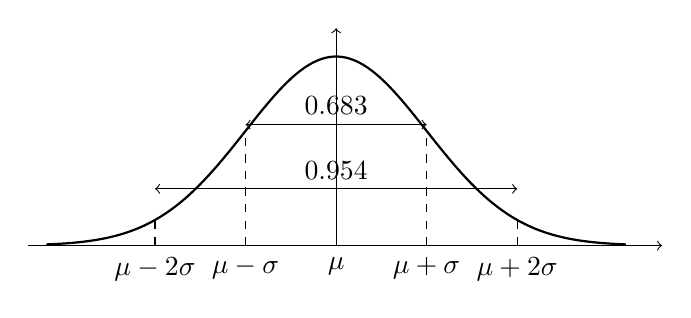
\begin{tikzpicture}[x=1.15cm,y=2.4cm]
  \draw[->] (-3.4,0) -- (3.6,0);
  \draw[->] (0,0) -- (0,1.15);
  \draw[thick,domain=-3.2:3.2,samples=120,smooth] plot (\x,{exp(-(\x*\x)/2)});
  \foreach \x in {-2,-1,1,2}
    \draw[dashed] (\x,0) -- (\x,{exp(-(\x*\x)/2)});
  \draw[dashed] (0,0) -- (0,1);
  \node[below] at (-2,-0.01) {$\mu-2\sigma$};
  \node[below] at (-1,-0.01) {$\mu-\sigma$};
  \node[below] at (0,-0.01) {$\mu$};
  \node[below] at (1,-0.01) {$\mu+\sigma$};
  \node[below] at (2,-0.01) {$\mu+2\sigma$};
  \draw[<->] (-1,0.64) -- (1,0.64) node[midway,above]{$0.683$};
  \draw[<->] (-2,0.30) -- (2,0.30) node[midway,above]{$0.954$};
\end{tikzpicture}
\phantomsection\label{fig:4.1}\mvcap{图 4.1\quad 具有均值 $\boldsymbol{\mu}$ 和方差 $\sigma^{2}$ 的正态密度及曲线下选定的面积}
\end{mvfigure}

用 $N(\mu,\sigma^{2})$ 表示具有均值 $\mu$ 和方差 $\sigma^{2}$ 的正态密度函数是方便的. 因此,$N(10,4)$ 表明\hyperref[eq:4-1]{式(4-1)}中的函数有 $\mu=10$ 和 $\sigma=2$. 这个表示法将扩展到以后的多元情况.
